\documentclass[tikz,border=3.14mm]{standalone}
\usepackage{amsmath}
\usetikzlibrary{matrix}
\begin{document}
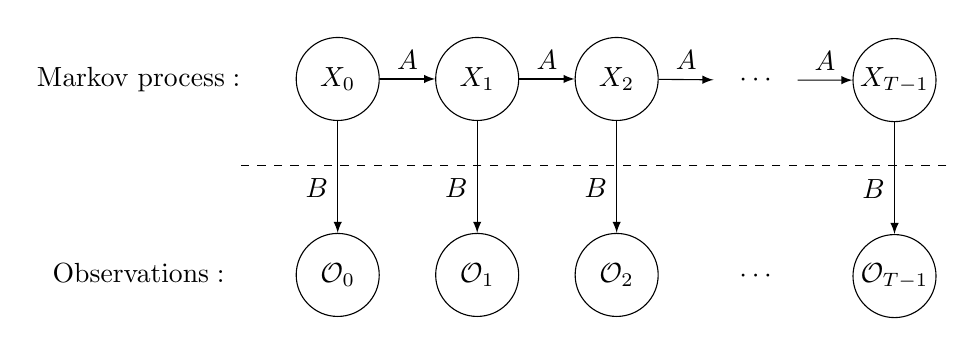
\begin{tikzpicture}
\matrix[matrix of math nodes,column sep=2em,row
sep=4em,cells={nodes={circle,draw,minimum width=3em,inner sep=0pt}},
column 1/.style={nodes={rectangle,draw=none}},
column 5/.style={nodes={rectangle,draw=none}}] (m) {
\text{Markov process}: &
 X_0 & X_1 & X_2 & \cdots & X_{T-1}\\
\text{Observations}: &
 \mathcal{O}_0 & \mathcal{O}_1 & \mathcal{O}_2 & \cdots & \mathcal{O}_{T-1}\\
};
\foreach \X in {2,3,4,5}
{\draw[-latex] (m-1-\X) -- (m-1-\the\numexpr\X+1) node[midway,above]{$A$};
\ifnum\X=5
\draw[-latex] (m-1-6) -- (m-2-6) node[pos=0.6,left]{$B$};
\else
\draw[-latex] (m-1-\X) -- (m-2-\X) node[pos=0.6,left]{$B$};
\fi}
\draw[dashed] ([yshift=1ex]m.east) -- ([yshift=1ex]m.east-|m-1-1.east);
\end{tikzpicture}
\end{document}
